% ------------------------------------------------------------------------------
% TYPO3 Version 10.4 - What's New (Serbian Version)
%
% @license	Creative Commons BY-NC-SA 3.0
% @link		https://typo3.org/help/documentation/whats-new/
% @language	Serbian
% ------------------------------------------------------------------------------

\section{Uvod}
\begin{frame}[fragile]
	\frametitle{Uvod}

	\begin{center}\huge{Uvod}\end{center}
	\begin{center}\huge{\color{typo3darkgrey}\textbf{Činjenice}}\end{center}

\end{frame}

% ------------------------------------------------------------------------------
% TYPO3 Version 10.4 - The Facts

\begin{frame}[fragile]
	\frametitle{Uvod}
	\framesubtitle{TYPO3 verzija 10.4 - Činjenice}

	\begin{itemize}
		\item Datum objavljivanja: 21. april 2020.
		\item Tip objavljivanja: LTS (objava sa dugoročnom podrškom)
	\end{itemize}

	\begin{figure}
		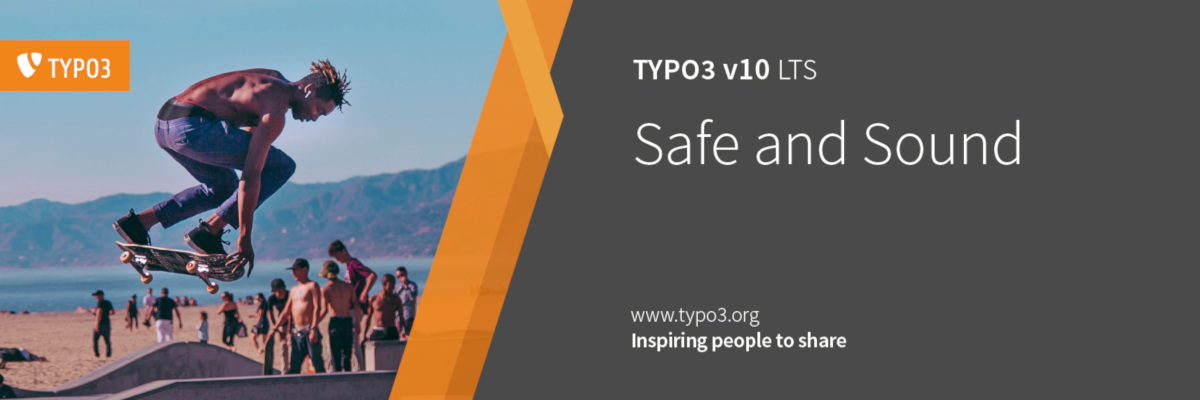
\includegraphics[width=0.95\linewidth]{Introduction/typo3-v10-4-banner.jpg}
	\end{figure}

\end{frame}

% ------------------------------------------------------------------------------
% TYPO3 Version 10.4 - Executive Summary

\begin{frame}[fragile]
	\frametitle{Uvod}
	\framesubtitle{Rezime}

	\small
		TYPO3 v10.4 (takodje se zove i TYPO3 v10 LTS označavajući da je ovo objava sa dugoročnom podrškom)
		je naš novi vodeći i bez sumnje jedan od najnaprednijih open-source sistema za upravljanje sadržajem
		na tržištu zasnovanih na PHP-u.

		\vspace{0.2cm}

		Nakon objavljivanja pet brzih objava od jula 2019. s ponosom možemo da kažemo
		da smo opremili TYPO3 sa najboljim PHP bibliotekama i da smo dodali još nekoliko
		fantastičnih naprednih funkcionalnosti.

		\vspace{0.2cm}

		Uzmite u obzir da ovaj dokument samo sumira izmene izmedju TYPO3 v10.3 i v10.4.

		\vspace{0.2cm}

		"What's New Slides" svih TYPO3 v10.x objava možete da pogledate na:
		\href{https://typo3.org/help/documentation/whats-new/}{typo3.org}.

	\normalsize

\end{frame}

% ------------------------------------------------------------------------------
% System Requirements

\begin{frame}[fragile]
	\frametitle{Uvod}
	\framesubtitle{Sistemski zahtevi}

	\begin{itemize}
		\item PHP verzija 7.2, 7.3 ili 7.4
		\item PHP podešavanja:

			\begin{itemize}
				\item \texttt{memory\_limit} >= 256M
				\item \texttt{max\_execution\_time} >= 240s
				\item \texttt{max\_input\_vars} >= 1500
				\item compilation option \texttt{-}\texttt{-disable-ipv6} must \underline{not} be used
			\end{itemize}

			\item Većina DB servera koji rade sa \textbf{Doctrine DBAL} rade takodje i sa TYPO3.
				Testirani DB serveri su:
	\end{itemize}

	\begin{figure}
		
\includegraphics[width=0.80\linewidth]{Introduction/logo-databases.png}
	\end{figure}

\end{frame}

% ------------------------------------------------------------------------------
% Development, Release, and Maintenance Timeline

\begin{frame}[fragile]
	\frametitle{Uvod}
	\framesubtitle{Razvoj, objavljivanje i vreme održavanja}

	\textbf{TYPO3 v10}

	\begin{figure}
		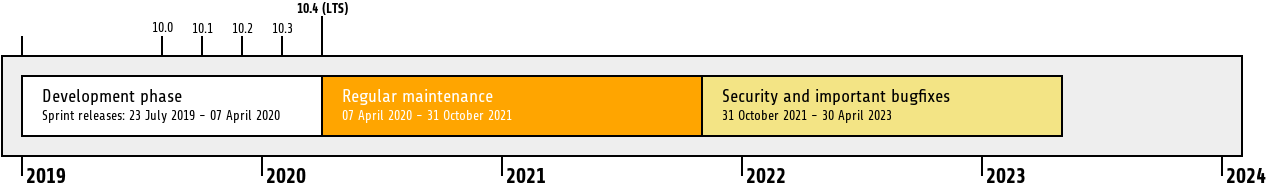
\includegraphics[width=1\linewidth]{Introduction/typo3-v10-lifecycle.png}
	\end{figure}

	\textbf{Produženo vreme podrške}\newline
	\smaller
		\href{https://typo3.com}{TYPO3 GmbH} nudi dodatne opcije za podršku za
		TYPO3 v10 LTS čak i posle 30. aprila 2023. za dodatne dve godine.
	\normalsize

\end{frame}

% ------------------------------------------------------------------------------
% TYPO3 v10 Roadmap

\begin{frame}[fragile]
	\frametitle{Uvod}
	\framesubtitle{TYPO3 v10 plan}

	Predvidjeni datumi objavljivanja i njihov osnovni fokus:

	\begin{itemize}

	\item v10.0 \tabto{1.1cm}23. jul 2019.\tabto{3.4cm}Otvaranje puta za uzbudljive nove koncepte i API-je
	\item v10.1 \tabto{1.1cm}01. okt. 2019.\tabto{3.4cm}Unapredjenje routing-a i upravljanje sajtom v2
	\item v10.2 \tabto{1.1cm}03. dec. 2019.\tabto{3.4cm}Fluid/Rendering Engine unapredjenja
		\item v10.3 \tabto{1.1cm}25. feb. 2020\tabto{3.4cm}Zamrzavanje funkcionalnosti
		\item
			\begingroup
				\color{typo3orange}
				v10.4 \tabto{1.1cm}21. apr. 2020\tabto{3.4cm}LTS objava (objava sa dugoročnom podrškom)
			\endgroup

	\end{itemize}

	\vspace{0.6cm}
	\smaller
		\url{https://typo3.org/article/typo3-v10-roadmap}\newline
		\url{https://typo3.org/article/typo3-v10-lts-safe-and-sound}
	\normalsize

\end{frame}

% ------------------------------------------------------------------------------
% Installation

\begin{frame}[fragile]
	\frametitle{Uvod}
	\framesubtitle{Instalacija}

	\begin{itemize}
	\item Zvanična \textit{klasična} procedura za instalaciju na Linux/Mac OS X
		(DocumentRoot na primer \texttt{/var/www/site/htdocs}):
\begin{lstlisting}
$ cd /var/www/site
$ wget --content-disposition get.typo3.org/10.4
$ tar xzf typo3_src-10.4.0.tar.gz
$ cd htdocs
$ ln -s ../typo3_src-10.4.0 typo3_src
$ ln -s typo3_src/index.php
$ ln -s typo3_src/typo3
$ touch FIRST_INSTALL
\end{lstlisting}

\item Simbolički linkovi (Symbolic links) na Microsoft Windows:

	\begin{itemize}
		\item Koristiti \texttt{junction} za Windows XP/2000
		\item Koristiti \texttt{mklink} za Windows Vista i Windows 7 i novije
	\end{itemize}

	\end{itemize}
\end{frame}

% ------------------------------------------------------------------------------
% Installation using composer

\begin{frame}[fragile]
	\frametitle{Installation and Upgrade}
	\framesubtitle{Instalacija korišćenjem \texttt{composer-a}}

	\begin{itemize}
		\item Instalacija korišćenjem \textit{composer-a} na Linux/Mac OS X i Windows 10:
\begin{lstlisting}
$ cd /var/www/site/
$ composer create-project typo3/cms-base-distribution typo3v10 ^10.4
\end{lstlisting}

		\item Alternativno, napravite Vaš \texttt{composer.json} fajl i pokrenite:
\begin{lstlisting}
$ composer install
\end{lstlisting}

			Više detalja vezano za Composer za TYPO3 jezgro i TYPO3 proširenja
			mozete pogledati ovde:

			\small
				\href{https://get.typo3.org/misc/composer/repository}{https://get.typo3.org/misc/composer/repository}
			\normalsize

	\end{itemize}
\end{frame}

% ------------------------------------------------------------------------------
